\documentclass[twoside]{book}

% Packages required by doxygen
\usepackage{fixltx2e}
\usepackage{calc}
\usepackage{doxygen}
\usepackage[export]{adjustbox} % also loads graphicx
\usepackage{graphicx}
\usepackage[utf8]{inputenc}
\usepackage{makeidx}
\usepackage{multicol}
\usepackage{multirow}
\PassOptionsToPackage{warn}{textcomp}
\usepackage{textcomp}
\usepackage[nointegrals]{wasysym}
\usepackage[table]{xcolor}

% Font selection
\usepackage[T1]{fontenc}
\usepackage[scaled=.90]{helvet}
\usepackage{courier}
\usepackage{amssymb}
\usepackage{sectsty}
\renewcommand{\familydefault}{\sfdefault}
\allsectionsfont{%
  \fontseries{bc}\selectfont%
  \color{darkgray}%
}
\renewcommand{\DoxyLabelFont}{%
  \fontseries{bc}\selectfont%
  \color{darkgray}%
}
\newcommand{\+}{\discretionary{\mbox{\scriptsize$\hookleftarrow$}}{}{}}

% Page & text layout
\usepackage{geometry}
\geometry{%
  a4paper,%
  top=2.5cm,%
  bottom=2.5cm,%
  left=2.5cm,%
  right=2.5cm%
}
\tolerance=750
\hfuzz=15pt
\hbadness=750
\setlength{\emergencystretch}{15pt}
\setlength{\parindent}{0cm}
\setlength{\parskip}{3ex plus 2ex minus 2ex}
\makeatletter
\renewcommand{\paragraph}{%
  \@startsection{paragraph}{4}{0ex}{-1.0ex}{1.0ex}{%
    \normalfont\normalsize\bfseries\SS@parafont%
  }%
}
\renewcommand{\subparagraph}{%
  \@startsection{subparagraph}{5}{0ex}{-1.0ex}{1.0ex}{%
    \normalfont\normalsize\bfseries\SS@subparafont%
  }%
}
\makeatother

% Headers & footers
\usepackage{fancyhdr}
\pagestyle{fancyplain}
\fancyhead[LE]{\fancyplain{}{\bfseries\thepage}}
\fancyhead[CE]{\fancyplain{}{}}
\fancyhead[RE]{\fancyplain{}{\bfseries\leftmark}}
\fancyhead[LO]{\fancyplain{}{\bfseries\rightmark}}
\fancyhead[CO]{\fancyplain{}{}}
\fancyhead[RO]{\fancyplain{}{\bfseries\thepage}}
\fancyfoot[LE]{\fancyplain{}{}}
\fancyfoot[CE]{\fancyplain{}{}}
\fancyfoot[RE]{\fancyplain{}{\bfseries\scriptsize Generated by Doxygen }}
\fancyfoot[LO]{\fancyplain{}{\bfseries\scriptsize Generated by Doxygen }}
\fancyfoot[CO]{\fancyplain{}{}}
\fancyfoot[RO]{\fancyplain{}{}}
\renewcommand{\footrulewidth}{0.4pt}
\renewcommand{\chaptermark}[1]{%
  \markboth{#1}{}%
}
\renewcommand{\sectionmark}[1]{%
  \markright{\thesection\ #1}%
}

% Indices & bibliography
\usepackage{natbib}
\usepackage[titles]{tocloft}
\setcounter{tocdepth}{3}
\setcounter{secnumdepth}{5}
\makeindex

% Hyperlinks (required, but should be loaded last)
\usepackage{ifpdf}
\ifpdf
  \usepackage[pdftex,pagebackref=true]{hyperref}
\else
  \usepackage[ps2pdf,pagebackref=true]{hyperref}
\fi
\hypersetup{%
  colorlinks=true,%
  linkcolor=blue,%
  citecolor=blue,%
  unicode%
}

% Custom commands
\newcommand{\clearemptydoublepage}{%
  \newpage{\pagestyle{empty}\cleardoublepage}%
}

\usepackage{caption}
\captionsetup{labelsep=space,justification=centering,font={bf},singlelinecheck=off,skip=4pt,position=top}

%===== C O N T E N T S =====

\begin{document}

% Titlepage & ToC
\hypersetup{pageanchor=false,
             bookmarksnumbered=true,
             pdfencoding=unicode
            }
\pagenumbering{roman}
\begin{titlepage}
\vspace*{7cm}
\begin{center}%
{\Large Lab2 }\\
\vspace*{1cm}
{\large Generated by Doxygen 1.8.11}\\
\end{center}
\end{titlepage}
\clearemptydoublepage
\tableofcontents
\clearemptydoublepage
\pagenumbering{arabic}
\hypersetup{pageanchor=true}

%--- Begin generated contents ---
\chapter{I\+E-\/0217-\/\+I\+I-\/16-\/\+Lab2-\/\+G2}
\label{md_README}
\hypertarget{md_README}{}
\input{md_README}
\chapter{Hierarchical Index}
\section{Class Hierarchy}
This inheritance list is sorted roughly, but not completely, alphabetically\+:\begin{DoxyCompactList}
\item \contentsline{section}{Figura}{\pageref{class_figura}}{}
\begin{DoxyCompactList}
\item \contentsline{section}{Circulo}{\pageref{class_circulo}}{}
\item \contentsline{section}{Cuadrado}{\pageref{class_cuadrado}}{}
\item \contentsline{section}{Triangulo}{\pageref{class_triangulo}}{}
\end{DoxyCompactList}
\end{DoxyCompactList}

\chapter{Class Index}
\section{Class List}
Here are the classes, structs, unions and interfaces with brief descriptions\+:\begin{DoxyCompactList}
\item\contentsline{section}{\hyperlink{class_calculadora}{Calculadora$<$ data $>$} }{\pageref{class_calculadora}}{}
\item\contentsline{section}{\hyperlink{class_fraccion}{Fraccion} }{\pageref{class_fraccion}}{}
\item\contentsline{section}{\hyperlink{class_matrix}{Matrix} }{\pageref{class_matrix}}{}
\item\contentsline{section}{\hyperlink{class_poly}{Poly} }{\pageref{class_poly}}{}
\end{DoxyCompactList}

\chapter{File Index}
\section{File List}
Here is a list of all documented files with brief descriptions\+:\begin{DoxyCompactList}
\item\contentsline{section}{\hyperlink{suma_8c}{suma.\+c} \\*Programa para sumar argumentos flotantes ingresados }{\pageref{suma_8c}}{}
\end{DoxyCompactList}

\chapter{Class Documentation}
\hypertarget{class_circulo}{}\section{Circulo Class Reference}
\label{class_circulo}\index{Circulo@{Circulo}}
Inheritance diagram for Circulo\+:\begin{figure}[H]
\begin{center}
\leavevmode
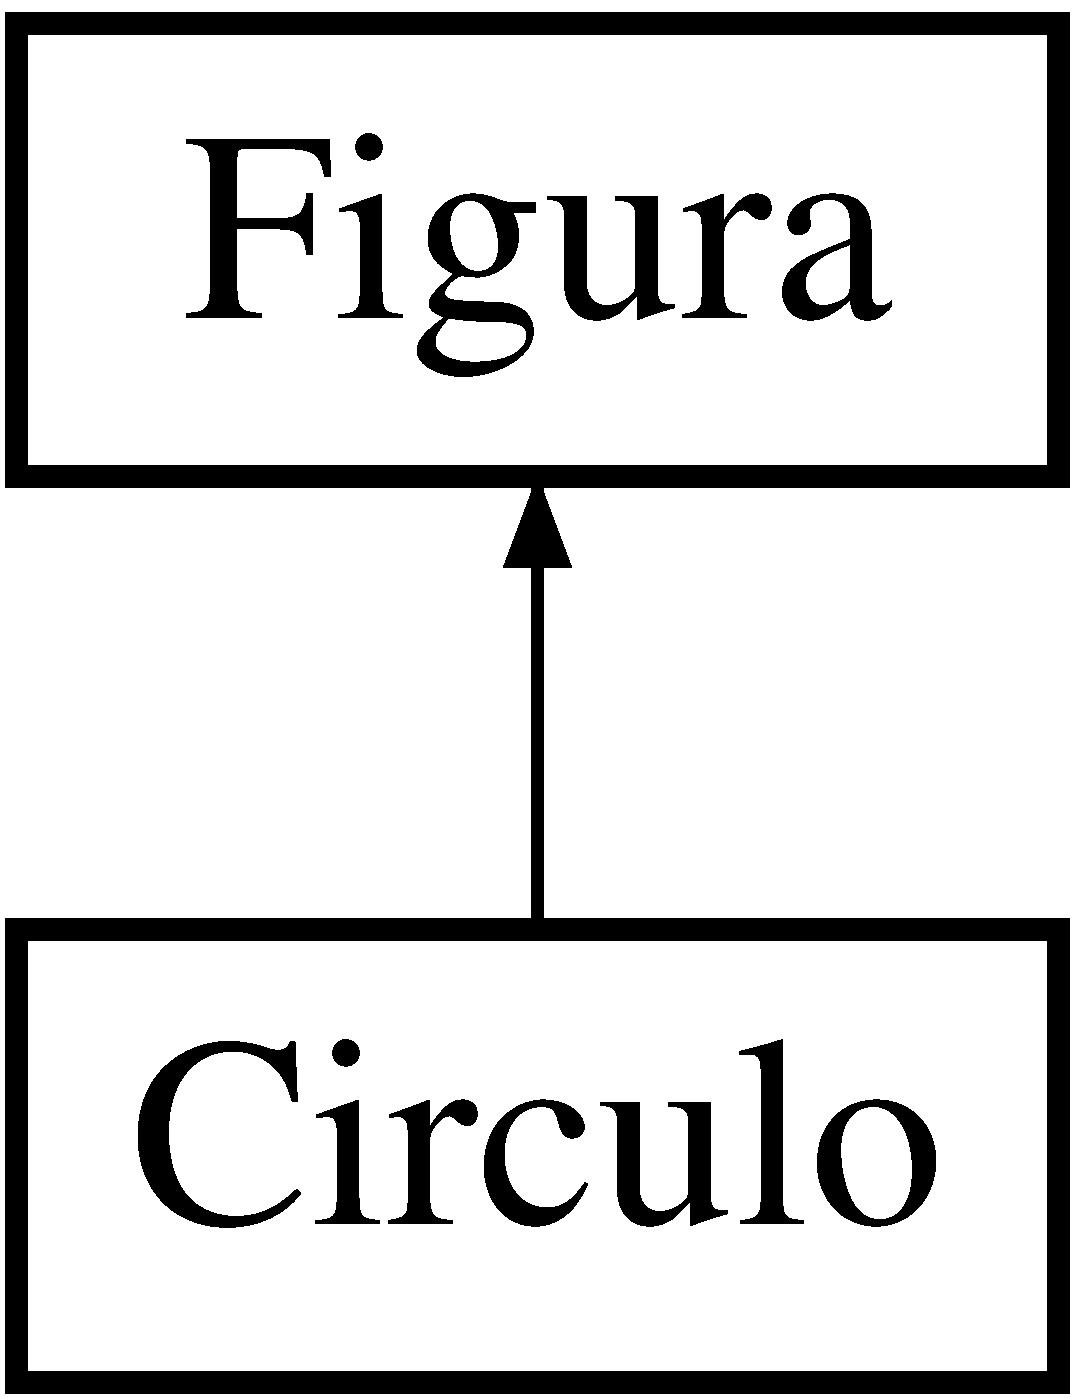
\includegraphics[height=2.000000cm]{class_circulo}
\end{center}
\end{figure}
\subsection*{Public Member Functions}
\begin{DoxyCompactItemize}
\item 
\hyperlink{class_circulo_a6933bf908b78a4167684081a3a8f257f}{Circulo} ()
\begin{DoxyCompactList}\small\item\em Me crea un circulo de radio ingresado por el usuario. \end{DoxyCompactList}\item 
{\bfseries Circulo} (std\+::string, std\+::string)\hypertarget{class_circulo_a966fa56f9f5262ebf4e33cbc094d07fd}{}\label{class_circulo_a966fa56f9f5262ebf4e33cbc094d07fd}

\item 
{\bfseries Circulo} (const \hyperlink{class_circulo}{Circulo} \&orig)\hypertarget{class_circulo_aa1ceac8b166daa79997baa338d6e37e5}{}\label{class_circulo_aa1ceac8b166daa79997baa338d6e37e5}

\item 
void {\bfseries Perimetro} ()\hypertarget{class_circulo_a4934591a9fffcc715527d45cd5035659}{}\label{class_circulo_a4934591a9fffcc715527d45cd5035659}

\item 
void {\bfseries Area} ()\hypertarget{class_circulo_a0796f73bbd8bf3206aa42222b243834f}{}\label{class_circulo_a0796f73bbd8bf3206aa42222b243834f}

\item 
void $\ast$ {\bfseries operator$\sim$} ()\hypertarget{class_circulo_a26b808c14a5bd66b12a7ebaa1dccf32c}{}\label{class_circulo_a26b808c14a5bd66b12a7ebaa1dccf32c}

\item 
void $\ast$ {\bfseries operator!} ()\hypertarget{class_circulo_a016704759e06464cc0413aaeb955cdd8}{}\label{class_circulo_a016704759e06464cc0413aaeb955cdd8}

\end{DoxyCompactItemize}
\subsection*{Public Attributes}
\begin{DoxyCompactItemize}
\item 
double {\bfseries radio}\hypertarget{class_circulo_aba57029c5768d344c4ef536e5323122b}{}\label{class_circulo_aba57029c5768d344c4ef536e5323122b}

\end{DoxyCompactItemize}


\subsection{Constructor \& Destructor Documentation}
\index{Circulo@{Circulo}!Circulo@{Circulo}}
\index{Circulo@{Circulo}!Circulo@{Circulo}}
\subsubsection[{\texorpdfstring{Circulo()}{Circulo()}}]{\setlength{\rightskip}{0pt plus 5cm}Circulo\+::\+Circulo (
\begin{DoxyParamCaption}
{}
\end{DoxyParamCaption}
)}\hypertarget{class_circulo_a6933bf908b78a4167684081a3a8f257f}{}\label{class_circulo_a6933bf908b78a4167684081a3a8f257f}


Me crea un circulo de radio ingresado por el usuario. 


\begin{DoxyParams}{Parameters}
{\em rad} & Valor del radio ingresado por el usuario \\
\hline
\end{DoxyParams}


The documentation for this class was generated from the following files\+:\begin{DoxyCompactItemize}
\item 
Circulo.\+h\item 
Circulo.\+cpp\end{DoxyCompactItemize}

\hypertarget{class_cuadrado}{}\section{Cuadrado Class Reference}
\label{class_cuadrado}\index{Cuadrado@{Cuadrado}}


{\ttfamily \#include $<$Cuadrado.\+h$>$}

Inheritance diagram for Cuadrado\+:\begin{figure}[H]
\begin{center}
\leavevmode
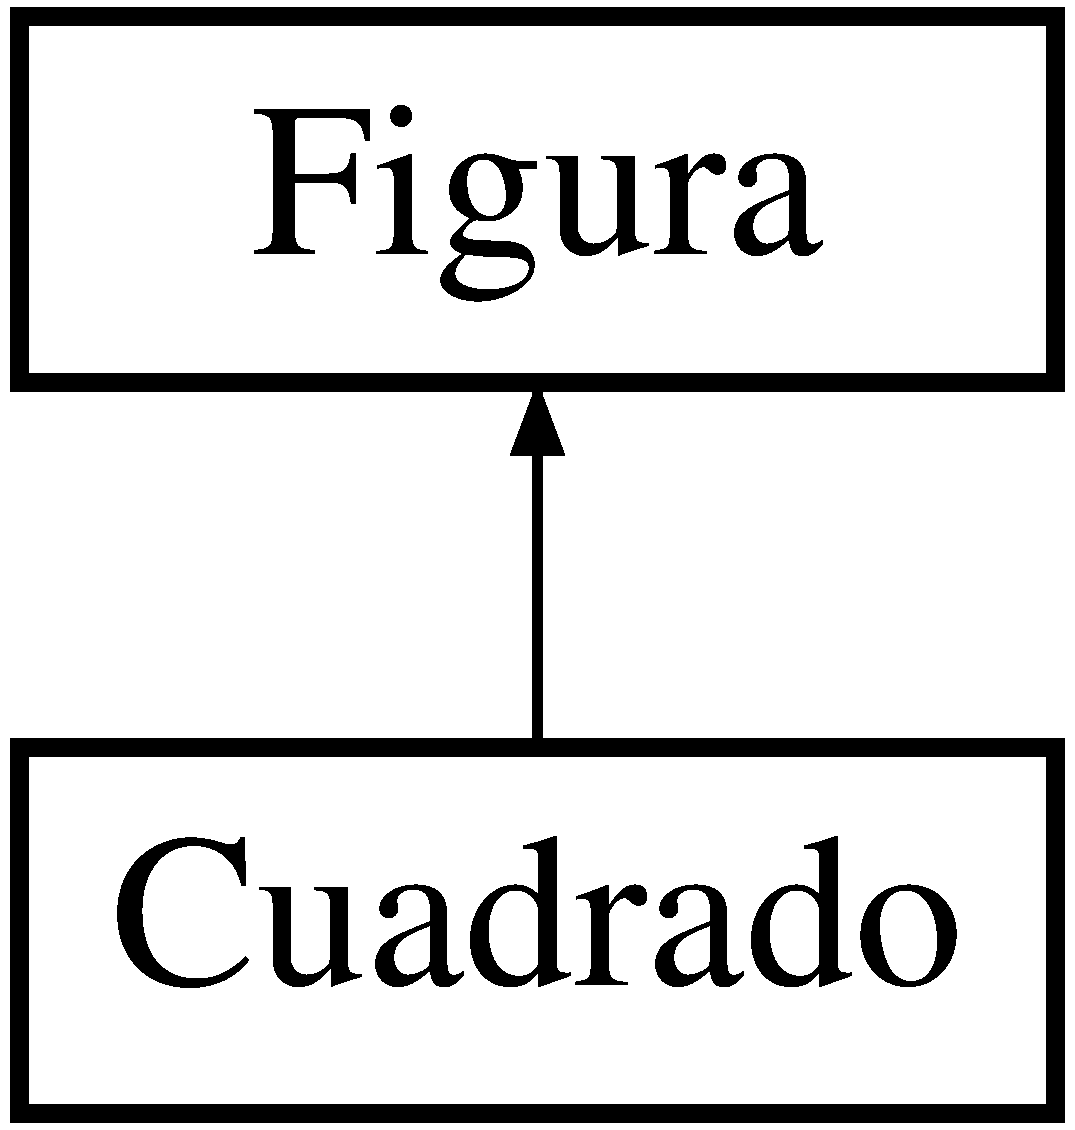
\includegraphics[height=2.000000cm]{class_cuadrado}
\end{center}
\end{figure}
\subsection*{Public Member Functions}
\begin{DoxyCompactItemize}
\item 
\hyperlink{class_cuadrado_ad28d9dddc29e1987ec620b07b0a4acc9}{Cuadrado} ()
\begin{DoxyCompactList}\small\item\em Me crea un cuadrado con un lado ingresado por el usuario. El constructor me genera un nombre y color genericos dado que en este caso no se le especifico algun nombre o color. \end{DoxyCompactList}\item 
\hyperlink{class_cuadrado_a1cdcb72a3c1475420599130e7488c6ad}{Cuadrado} (std\+::string, std\+::string)
\begin{DoxyCompactList}\small\item\em Genera un cuadrado con nombre y color ingresado por el usuario con una longitud del lado ingresado por el usuario. \end{DoxyCompactList}\item 
{\bfseries Cuadrado} (const \hyperlink{class_cuadrado}{Cuadrado} \&orig)\hypertarget{class_cuadrado_a51f15bc1eb52008d394ac1191e257aeb}{}\label{class_cuadrado_a51f15bc1eb52008d394ac1191e257aeb}

\item 
void \hyperlink{class_cuadrado_a3d1411d7a4cd8734938092727009d702}{Area} ()
\begin{DoxyCompactList}\small\item\em Funcion para calcular el area del cuadrado. \end{DoxyCompactList}\item 
void \hyperlink{class_cuadrado_aa1b3dceb0c4ecfe7680f459c635e6d28}{Perimetro} ()
\begin{DoxyCompactList}\small\item\em Funcion para calcular el perimetro del cuadrado. \end{DoxyCompactList}\item 
void $\ast$ \hyperlink{class_cuadrado_a8600ccace0a61a8ba7dd0933bd344b33}{operator$\sim$} ()
\begin{DoxyCompactList}\small\item\em Muestra las propiedades del cuadrado. \end{DoxyCompactList}\item 
void $\ast$ \hyperlink{class_cuadrado_af911d1931dba68c5ed410852569f365b}{operator!} ()
\begin{DoxyCompactList}\small\item\em Muestra el resultado del calculo de area y perimetro. \end{DoxyCompactList}\end{DoxyCompactItemize}
\subsection*{Public Attributes}
\begin{DoxyCompactItemize}
\item 
double {\bfseries lado}\hypertarget{class_cuadrado_a0480679f3e1c059282f532167c81d439}{}\label{class_cuadrado_a0480679f3e1c059282f532167c81d439}

\end{DoxyCompactItemize}


\subsection{Detailed Description}
\+: \hyperlink{_cuadrado_8h_source}{Cuadrado.\+h} \begin{DoxyAuthor}{Author}
\+: jose
\end{DoxyAuthor}
\begin{DoxyDate}{Date}
September 6, 2016 
\end{DoxyDate}

\begin{DoxyParams}{Parameters}
{\em lado} & guarda el lado de cada cuadrado creado \\
\hline
\end{DoxyParams}


\subsection{Constructor \& Destructor Documentation}
\index{Cuadrado@{Cuadrado}!Cuadrado@{Cuadrado}}
\index{Cuadrado@{Cuadrado}!Cuadrado@{Cuadrado}}
\subsubsection[{\texorpdfstring{Cuadrado()}{Cuadrado()}}]{\setlength{\rightskip}{0pt plus 5cm}Cuadrado\+::\+Cuadrado (
\begin{DoxyParamCaption}
{}
\end{DoxyParamCaption}
)}\hypertarget{class_cuadrado_ad28d9dddc29e1987ec620b07b0a4acc9}{}\label{class_cuadrado_ad28d9dddc29e1987ec620b07b0a4acc9}


Me crea un cuadrado con un lado ingresado por el usuario. El constructor me genera un nombre y color genericos dado que en este caso no se le especifico algun nombre o color. 


\begin{DoxyParams}{Parameters}
{\em l} & variable temporal para guardar el lado. \\
\hline
\end{DoxyParams}
\index{Cuadrado@{Cuadrado}!Cuadrado@{Cuadrado}}
\index{Cuadrado@{Cuadrado}!Cuadrado@{Cuadrado}}
\subsubsection[{\texorpdfstring{Cuadrado(std\+::string, std\+::string)}{Cuadrado(std::string, std::string)}}]{\setlength{\rightskip}{0pt plus 5cm}Cuadrado\+::\+Cuadrado (
\begin{DoxyParamCaption}
\item[{std\+::string}]{a, }
\item[{std\+::string}]{b}
\end{DoxyParamCaption}
)}\hypertarget{class_cuadrado_a1cdcb72a3c1475420599130e7488c6ad}{}\label{class_cuadrado_a1cdcb72a3c1475420599130e7488c6ad}


Genera un cuadrado con nombre y color ingresado por el usuario con una longitud del lado ingresado por el usuario. 


\begin{DoxyParams}{Parameters}
{\em a} & Guarda el nombre temporalmente \\
\hline
{\em b} & Guarda el color temporalmente 
\begin{DoxyCode}
this->color = b; 
this->nombre = a;
\end{DoxyCode}
 \\
\hline
\end{DoxyParams}


\subsection{Member Function Documentation}
\index{Cuadrado@{Cuadrado}!Area@{Area}}
\index{Area@{Area}!Cuadrado@{Cuadrado}}
\subsubsection[{\texorpdfstring{Area()}{Area()}}]{\setlength{\rightskip}{0pt plus 5cm}void Cuadrado\+::\+Area (
\begin{DoxyParamCaption}
{}
\end{DoxyParamCaption}
)\hspace{0.3cm}{\ttfamily [virtual]}}\hypertarget{class_cuadrado_a3d1411d7a4cd8734938092727009d702}{}\label{class_cuadrado_a3d1411d7a4cd8734938092727009d702}


Funcion para calcular el area del cuadrado. 


\begin{DoxyCode}
\textcolor{keywordtype}{double} area = this->lado * this->lado ; 
\end{DoxyCode}
 
\begin{DoxyParams}{Parameters}
{\em area} & Variable temporal del metodo para el area del cuadrado \\
\hline
\end{DoxyParams}


Implements \hyperlink{class_figura}{Figura}.

\index{Cuadrado@{Cuadrado}!operator"!@{operator"!}}
\index{operator"!@{operator"!}!Cuadrado@{Cuadrado}}
\subsubsection[{\texorpdfstring{operator"!()}{operator!()}}]{\setlength{\rightskip}{0pt plus 5cm}void $\ast$ Cuadrado\+::operator! (
\begin{DoxyParamCaption}
{}
\end{DoxyParamCaption}
)}\hypertarget{class_cuadrado_af911d1931dba68c5ed410852569f365b}{}\label{class_cuadrado_af911d1931dba68c5ed410852569f365b}


Muestra el resultado del calculo de area y perimetro. 

\begin{DoxyReturn}{Returns}
No retorna nada ademas de imprimir la informacion. 
\end{DoxyReturn}
\index{Cuadrado@{Cuadrado}!operator````~@{operator$\sim$}}
\index{operator````~@{operator$\sim$}!Cuadrado@{Cuadrado}}
\subsubsection[{\texorpdfstring{operator$\sim$()}{operator~()}}]{\setlength{\rightskip}{0pt plus 5cm}void $\ast$ Cuadrado\+::operator$\sim$ (
\begin{DoxyParamCaption}
{}
\end{DoxyParamCaption}
)}\hypertarget{class_cuadrado_a8600ccace0a61a8ba7dd0933bd344b33}{}\label{class_cuadrado_a8600ccace0a61a8ba7dd0933bd344b33}


Muestra las propiedades del cuadrado. 

\begin{DoxyReturn}{Returns}
No retorna nada ademas de imprimir la informacion 
\end{DoxyReturn}
\index{Cuadrado@{Cuadrado}!Perimetro@{Perimetro}}
\index{Perimetro@{Perimetro}!Cuadrado@{Cuadrado}}
\subsubsection[{\texorpdfstring{Perimetro()}{Perimetro()}}]{\setlength{\rightskip}{0pt plus 5cm}void Cuadrado\+::\+Perimetro (
\begin{DoxyParamCaption}
{}
\end{DoxyParamCaption}
)\hspace{0.3cm}{\ttfamily [virtual]}}\hypertarget{class_cuadrado_aa1b3dceb0c4ecfe7680f459c635e6d28}{}\label{class_cuadrado_aa1b3dceb0c4ecfe7680f459c635e6d28}


Funcion para calcular el perimetro del cuadrado. 


\begin{DoxyParams}{Parameters}
{\em Per} & guarda el resultado del calculo del perimetro. \\
\hline
\end{DoxyParams}


Implements \hyperlink{class_figura}{Figura}.



The documentation for this class was generated from the following files\+:\begin{DoxyCompactItemize}
\item 
Cuadrado.\+h\item 
Cuadrado.\+cpp\end{DoxyCompactItemize}

\hypertarget{class_figura}{}\section{Figura Class Reference}
\label{class_figura}\index{Figura@{Figura}}
Inheritance diagram for Figura\+:\begin{figure}[H]
\begin{center}
\leavevmode
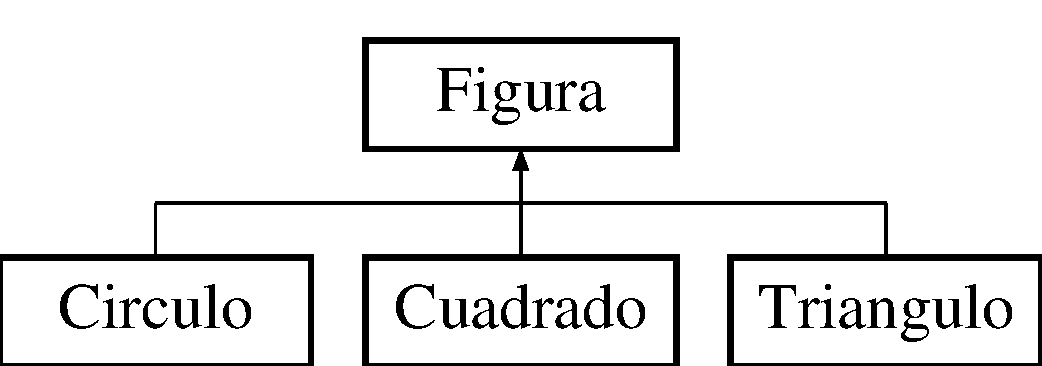
\includegraphics[height=2.000000cm]{class_figura}
\end{center}
\end{figure}
\subsection*{Public Member Functions}
\begin{DoxyCompactItemize}
\item 
{\bfseries Figura} (const \hyperlink{class_figura}{Figura} \&orig)\hypertarget{class_figura_aa50330af66b067bd5e7d905075a2ccd6}{}\label{class_figura_aa50330af66b067bd5e7d905075a2ccd6}

\item 
virtual void {\bfseries Area} ()=0\hypertarget{class_figura_aa962385ee2648a5241c9ded07af162f7}{}\label{class_figura_aa962385ee2648a5241c9ded07af162f7}

\item 
virtual void {\bfseries Perimetro} ()=0\hypertarget{class_figura_a464ba53b8842754284bf552d3a1fbf26}{}\label{class_figura_a464ba53b8842754284bf552d3a1fbf26}

\end{DoxyCompactItemize}
\subsection*{Public Attributes}
\begin{DoxyCompactItemize}
\item 
std\+::string {\bfseries nombre}\hypertarget{class_figura_a67df59705ff131e5a56fe4d4af3cfb73}{}\label{class_figura_a67df59705ff131e5a56fe4d4af3cfb73}

\item 
std\+::string {\bfseries color}\hypertarget{class_figura_ab27a1a9f1236ad5ce14fce5776ed3aea}{}\label{class_figura_ab27a1a9f1236ad5ce14fce5776ed3aea}

\item 
double {\bfseries area}\hypertarget{class_figura_a80031f56cf5f383824012b2256d0334d}{}\label{class_figura_a80031f56cf5f383824012b2256d0334d}

\item 
double {\bfseries perimetro}\hypertarget{class_figura_a726780324c8107f9ac6915aa6be80966}{}\label{class_figura_a726780324c8107f9ac6915aa6be80966}

\end{DoxyCompactItemize}


The documentation for this class was generated from the following files\+:\begin{DoxyCompactItemize}
\item 
Figura.\+h\item 
Figura.\+cpp\end{DoxyCompactItemize}

\hypertarget{class_triangulo}{}\section{Triangulo Class Reference}
\label{class_triangulo}\index{Triangulo@{Triangulo}}
Inheritance diagram for Triangulo\+:\begin{figure}[H]
\begin{center}
\leavevmode
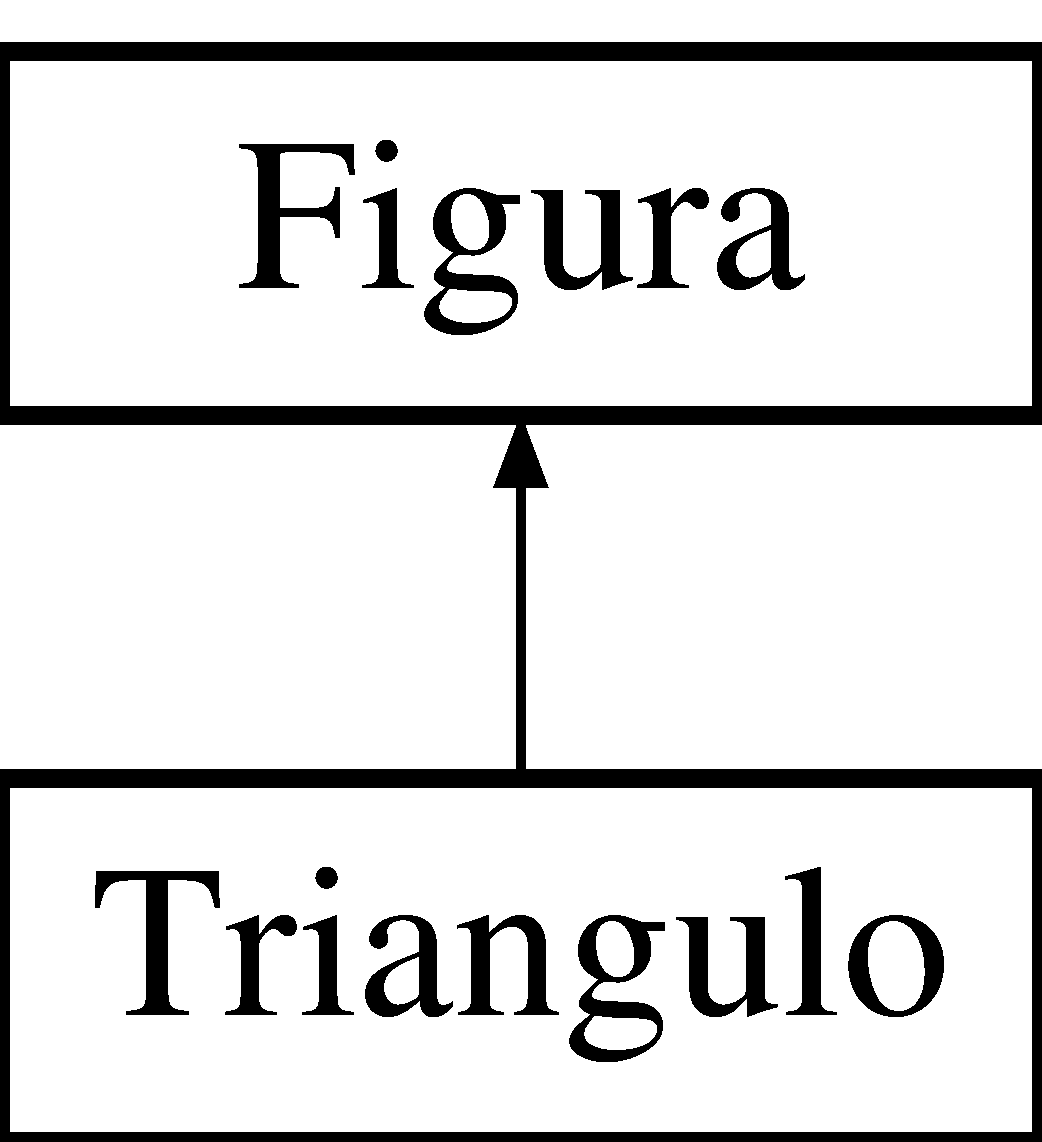
\includegraphics[height=2.000000cm]{class_triangulo}
\end{center}
\end{figure}
\subsection*{Public Member Functions}
\begin{DoxyCompactItemize}
\item 
\hyperlink{class_triangulo_a905d421bd19655a979ccad9e2998db0c}{Triangulo} ()\hypertarget{class_triangulo_a905d421bd19655a979ccad9e2998db0c}{}\label{class_triangulo_a905d421bd19655a979ccad9e2998db0c}

\begin{DoxyCompactList}\small\item\em Me crea un triangulo con nombre y color genericos. \end{DoxyCompactList}\item 
{\bfseries Triangulo} (const \hyperlink{class_triangulo}{Triangulo} \&orig)\hypertarget{class_triangulo_a1a7267ad3feb850a9718002420fc2fd8}{}\label{class_triangulo_a1a7267ad3feb850a9718002420fc2fd8}

\item 
\hyperlink{class_triangulo_aa56f00477a32f8c6465b2b7256fdd7d0}{Triangulo} (std\+::string, std\+::string)
\begin{DoxyCompactList}\small\item\em Me crea un triangulo con nombre y color ingresado por el usuario. \end{DoxyCompactList}\item 
void \hyperlink{class_triangulo_a1174be9286bedca30ef95806c52bdc2d}{obtener\+Lados} ()\hypertarget{class_triangulo_a1174be9286bedca30ef95806c52bdc2d}{}\label{class_triangulo_a1174be9286bedca30ef95806c52bdc2d}

\begin{DoxyCompactList}\small\item\em Obtiene los lado del triangulo (tres lados) y los guarda en los lados de cada triangulo creado (this-\/$>$lado). \end{DoxyCompactList}\item 
void {\bfseries Area} ()\hypertarget{class_triangulo_aa8d4fae608682df1bcac3b68982a86e6}{}\label{class_triangulo_aa8d4fae608682df1bcac3b68982a86e6}

\item 
void {\bfseries Perimetro} ()\hypertarget{class_triangulo_a02c05bf39e881390e7bc9bf3d6f1b680}{}\label{class_triangulo_a02c05bf39e881390e7bc9bf3d6f1b680}

\item 
void $\ast$ \hyperlink{class_triangulo_a7a8a19fd43cb3181e672b004b4ce83d5}{operator$\sim$} ()
\begin{DoxyCompactList}\small\item\em Muestra los atributos de cada triangulo (nombre, color, lados). \end{DoxyCompactList}\item 
void $\ast$ \hyperlink{class_triangulo_ab234082ba67e5dd0636b05e24884c470}{operator!} ()
\begin{DoxyCompactList}\small\item\em Muestra los resultados de area y perimetro. \end{DoxyCompactList}\end{DoxyCompactItemize}
\subsection*{Public Attributes}
\begin{DoxyCompactItemize}
\item 
double {\bfseries lado1}\hypertarget{class_triangulo_ad56af20f632db44b7bd02b9435d6d979}{}\label{class_triangulo_ad56af20f632db44b7bd02b9435d6d979}

\item 
double {\bfseries lado2}\hypertarget{class_triangulo_ae76fdab53758e4786e8f8cb2640c8bf7}{}\label{class_triangulo_ae76fdab53758e4786e8f8cb2640c8bf7}

\item 
double {\bfseries lado3}\hypertarget{class_triangulo_a4c6887a4f81fe2b6afc940d52e75b2bc}{}\label{class_triangulo_a4c6887a4f81fe2b6afc940d52e75b2bc}

\end{DoxyCompactItemize}


\subsection{Constructor \& Destructor Documentation}
\index{Triangulo@{Triangulo}!Triangulo@{Triangulo}}
\index{Triangulo@{Triangulo}!Triangulo@{Triangulo}}
\subsubsection[{\texorpdfstring{Triangulo(std\+::string, std\+::string)}{Triangulo(std::string, std::string)}}]{\setlength{\rightskip}{0pt plus 5cm}Triangulo\+::\+Triangulo (
\begin{DoxyParamCaption}
\item[{std\+::string}]{a, }
\item[{std\+::string}]{b}
\end{DoxyParamCaption}
)}\hypertarget{class_triangulo_aa56f00477a32f8c6465b2b7256fdd7d0}{}\label{class_triangulo_aa56f00477a32f8c6465b2b7256fdd7d0}


Me crea un triangulo con nombre y color ingresado por el usuario. 


\begin{DoxyCode}
this->nombre = a; 
this->color = b;
\hyperlink{class_triangulo_a1174be9286bedca30ef95806c52bdc2d}{Triangulo::obtenerLados}();
\end{DoxyCode}
 
\begin{DoxyParams}{Parameters}
{\em a} & Nombre del triangulo \\
\hline
{\em b} & Color del triangulo \\
\hline
\end{DoxyParams}


\subsection{Member Function Documentation}
\index{Triangulo@{Triangulo}!operator"!@{operator"!}}
\index{operator"!@{operator"!}!Triangulo@{Triangulo}}
\subsubsection[{\texorpdfstring{operator"!()}{operator!()}}]{\setlength{\rightskip}{0pt plus 5cm}void $\ast$ Triangulo\+::operator! (
\begin{DoxyParamCaption}
{}
\end{DoxyParamCaption}
)}\hypertarget{class_triangulo_ab234082ba67e5dd0636b05e24884c470}{}\label{class_triangulo_ab234082ba67e5dd0636b05e24884c470}


Muestra los resultados de area y perimetro. 

\begin{DoxyReturn}{Returns}
Informacion 
\end{DoxyReturn}
\index{Triangulo@{Triangulo}!operator````~@{operator$\sim$}}
\index{operator````~@{operator$\sim$}!Triangulo@{Triangulo}}
\subsubsection[{\texorpdfstring{operator$\sim$()}{operator~()}}]{\setlength{\rightskip}{0pt plus 5cm}void $\ast$ Triangulo\+::operator$\sim$ (
\begin{DoxyParamCaption}
{}
\end{DoxyParamCaption}
)}\hypertarget{class_triangulo_a7a8a19fd43cb3181e672b004b4ce83d5}{}\label{class_triangulo_a7a8a19fd43cb3181e672b004b4ce83d5}


Muestra los atributos de cada triangulo (nombre, color, lados). 

\begin{DoxyReturn}{Returns}
Informacion 
\end{DoxyReturn}


The documentation for this class was generated from the following files\+:\begin{DoxyCompactItemize}
\item 
Triangulo.\+h\item 
Triangulo.\+cpp\end{DoxyCompactItemize}

\chapter{File Documentation}
\hypertarget{main_8cpp}{}\section{main.\+cpp File Reference}
\label{main_8cpp}\index{main.\+cpp@{main.\+cpp}}


Main donde se encuentran las pruebas de la clase figura y sus subclases por herencia.  


{\ttfamily \#include \char`\"{}Figura.\+h\char`\"{}}\\*
{\ttfamily \#include \char`\"{}Triangulo.\+h\char`\"{}}\\*
{\ttfamily \#include \char`\"{}Circulo.\+h\char`\"{}}\\*
{\ttfamily \#include \char`\"{}Cuadrado.\+h\char`\"{}}\\*
\subsection*{Functions}
\begin{DoxyCompactItemize}
\item 
int {\bfseries main} (int argc, char $\ast$$\ast$argv)\hypertarget{main_8cpp_a3c04138a5bfe5d72780bb7e82a18e627}{}\label{main_8cpp_a3c04138a5bfe5d72780bb7e82a18e627}

\end{DoxyCompactItemize}


\subsection{Detailed Description}
Main donde se encuentran las pruebas de la clase figura y sus subclases por herencia. 

\begin{DoxyAuthor}{Author}
Jose Alberto Barrantes 
\end{DoxyAuthor}
\begin{DoxyDate}{Date}
9 Sep 2016. 
\end{DoxyDate}

%--- End generated contents ---

% Index
\backmatter
\newpage
\phantomsection
\clearemptydoublepage
\addcontentsline{toc}{chapter}{Index}
\printindex

\end{document}
